\begin{abstract}
本文检验公开四维形成渠道模型如何一致接入含有额外自旋坐标的事件后验与搜索注入。我们保留固定的69个GWTC-3时期观测及全部11,180,578行已恢复来源的后验。在明确限制的质量、红移和自旋域内，将五个公开渠道模拟器固定于出生自旋0.1、共同包层效率2，比较两种显式隐藏自旋条件补全、三个正则化概率、两份O3注入银行和两种搜索口径，共24组条件后验。内禀分支中位数沿这四个比较轴的最大移动分别为\MaxHidden、\MaxReg、\MaxBank、\MaxPolicy\ 个百分点；两套独立后验算法的已核查分位数相差不超过\MaxIndependent\ 个百分点。由于共同均匀项的计算效率远高于共同包层模型，1\%的密度正则项可占检出模型混合约12\%。这些结果是固定保存银行上的条件敏感性研究，不是宇宙形成比例测量，也未认证历史检出协议。事件和注入贡献集中的问题仍构成重要未决误差。
\end{abstract}

\section{问题及其与已有研究的关系}
群体合成把黑洞形成情景连接到可观测双星参数分布。多渠道推断、归一化流模拟器、Dirichlet分支先验与尾部正则化均已用于已有研究\cite{zevin,colloms}；实现它们不构成新的推断方法。这里的问题更具体：当发布模型只预测源系啁啾质量、质量比、有效自旋和红移时，一致的事件与选择计算还需要怎样的分量自旋分布，这个补充假设会怎样改变分支权重？

固定有效自旋并不能唯一确定分量自旋，这一点已有研究。Miller等\cite{miller}用有效自旋分布相同、分量自旋不同的模拟总体做完整推断；Spinformation\cite{plunkett}进一步给出条件先验和有效参数之外的信息量诊断。有效自旋先验及联合先验精度也有现成研究\cite{callister,iwaya}。本文不主张发现新的退化关系、先验公式或信息量检验；增量限于在同一组恢复来源的事件与官方注入银行上，传播两个明确条件补全，并保存完整乘积和原始数值失败。

\section{数据与条件实验}
分析保留此前工作台全来源研究的同一69个观测。事件身份、分析标签、先验族和缓存哈希从公开GWTC-2.1与GWTC-3后验发布中恢复。全部11,180,578行都用于积分，不删除高权重样本或事件。事件先验在原生七坐标表示中计算，只省略在比较模型间共同的事件级常数。已恢复保存行上的密度，不等于已知道原PE先验排除区域的似然。

五个渠道分别是共同包层演化（CE）、化学均匀演化（CHE）、球状星团（GC）、核星团（NSC）和稳定质量转移（SMT）。数值流权重与映射来自文献\cite{colloms}关联的CC BY 4.0数据发布。原创适配器通过Glasflow严格读取张量state dictionary；下载的AMAZE源码只检查，不执行或再分发。CE使用$[\chi_b,\ln\alpha_{\rm CE}]$上下文。公开参考样本的诊断支持这一解释优于直接线性alpha上下文，但尚未重建历史训练调用。

我们固定$\chi_b=0.1$、$\alpha_{\rm CE}=2$。采用源系太阳质量单位，限制域为
\begin{equation}\label{eq:domain}
D:\quad 5\le m_1\le100,\quad m_2\ge3,\quad q\le1,\quad0<z\le1.9,\quad |\ceff|<A,\quad A=0.99.
\end{equation}
补全分布的两颗自旋幅度也小于$A$。这是限制域实验，不是全宇宙总体推断。GC公开映射允许$q<1.001$；$q>1$样本保留计数，在明确的域指示函数下不贡献归一化，不做折叠或裁剪。

每渠道使用262,144个独立潜变量正态抽样估计域归一化$Z_c$。CE、CHE、GC、NSC、SMT分别约为0.33539、0.61481、0.66197、0.77760、0.68363；各自Bernoulli MC标准误约为$0.0008$至$0.0010$。它们是模拟器的域概率，不是检出效率或已经认证的物理支持率。

\section{显式的四维到七维提升}
记$\theta=(\mathcal M,q,x,z)$，$x=\ceff$，$s=(a_1,a_2,c_1,c_2)$，其中$c_i=\cos\tau_i$。有
\begin{equation}\label{eq:spin}
x=\frac{a_1c_1+q a_2c_2}{1+q},\qquad
J(q)=\frac{d m_1}{d\mathcal M}=\frac{(1+q)^{1/5}}{q^{3/5}}.
\end{equation}
设$Q(s)$为归一化基准自旋律，$f_Q(x\mid q)$为其有效自旋边缘，定义
\begin{equation}\label{eq:lift}
p_{7,c}=\frac{\ind_D\,p_{4,c}(\mathcal M,q,x,z)}{Z_c J(q)}\,
\frac{Q(s)}{f_Q(x\mid q)}.
\end{equation}
积分掉未建模自旋后，还原$\ind_Dp_{4,c}/Z_c$。因此，不同条件律可以保留完全相同的四维预测，同时给出不同的完整自旋模型。方位角均匀性隐含在角度边缘化中。这是明确新增的假设，不是四维模拟器已经提供的物理。

我们用两颗独立、方向各向同性的自旋作为基准律，幅度分别取$[0,A]$上的均匀分布或缩放Beta$(2,5)$。单体轴向投影为
\begin{equation}\label{eq:axial}
f_U(s_z)=\frac{\ln(A/|s_z|)}{2A},\qquad
f_B(s_z)=\frac{3}{A}\left(1-\frac{|s_z|}{A}\right)^5,\quad |s_z|<A.
\end{equation}
一维卷积给出$f_Q(x\mid q)$；均匀幅度结果与已有先验计算一致\cite{callister}。提升后的总体幅度边缘一般不再是原来的均匀或Beta分布；两种补全也没有被认定为CE、GC等渠道的真实分量自旋预测。

当缩放事件先验$\pi_7=\pi_{m,z}Q_U$时，相应四维先验是
\begin{equation}\label{eq:reduced}
\pi_4=4A^2 J(q) f_U(x\mid q)\,\pi_7.
\end{equation}
均匀补全因而还原四维边缘先验下的重要性权重；直接以四维渠道密度除以$\pi_7$不成立。对于Cartesian注入，坐标因子为$m_1(2\pi a_1^2)(2\pi a_2^2)$，保留发布的联合提议密度。两种基准律都一致用于PE和注入权重。

\section{选择、正则化与分支量的定义}
O3两种表示分别为完整纯BBH银行和官方四总体混合银行。比较匹配滤波IFAR并集与包含cWB的另一并集，O1/O2条件计算保持此前定义。积分包含发布的生成总数、混合权重和观测时间因子。独立银行审计核对精确来源连接，但没有恢复全部历史筛选、自旋参考和执行协议。

令$A_{ic}$为式\eqref{eq:lift}的全行事件均值，$\xi_c$为合并选择积分，$N=69$，$\sum_c\beta_c=1$，则
\begin{equation}\label{eq:likelihood}
\mathcal L(\bm\beta)\propto
\frac{\prod_{i=1}^N\sum_c\beta_c A_{ic}}
{\left(\sum_c\beta_c\xi_c\right)^N},\qquad
\bm\beta\sim\operatorname{Dirichlet}(1,1,1,1,1).
\end{equation}
先验定义在\emph{域$D$内}的内禀比例上。域外样本目标权重为零，但仍保留在事件均值的分母中。

沿用文献\cite{colloms}关于尾部不可靠性的动机，测试$\epsilon\in\{0,0.001,0.01\}$。共同正则器$U$在$D$内的$(m_1,q,z,x)$坐标中为常数，质量面积为$95-3\ln20$；换到$\mathcal M$时包含$J(q)$。其提升采用与渠道一致的条件自旋律，同时进入两项：
\begin{equation}\label{eq:regularization}
A_{ic}'=(1-\epsilon)A_{ic}+\epsilon U_i,
\qquad \xi_c'=(1-\epsilon)\xi_c+\epsilon\xi_U.
\end{equation}
两个自旋补全、两份银行、两搜索口径、三个正则器形成24组拟合。这个指定网格不是模型平均，也不是全部模型误差的可信包络。

检出标签权重为
\begin{equation}\label{eq:label}
\eta_c^{\rm label}=\frac{\beta_c\xi_c'}{\xi'},\qquad
\xi'=(1-\epsilon)\sum_d\beta_d\xi_d+\epsilon\xi_U.
\end{equation}
由于$U$共同，这种约定把它按$\bm\beta$分配给各渠道标签。为避免物理解读混淆，另报告
\begin{equation}\label{eq:decomposition}
\eta_c^{\rm model}=\frac{(1-\epsilon)\beta_c\xi_c}{\xi'},\quad
w_U=\frac{\epsilon\xi_U}{\xi'},\quad
\eta_c^{\rm label}=\eta_c^{\rm model}+\beta_c w_U.
\end{equation}
五个模型项与$w_U$共同加和为1。$w_U$只是数学责任份额，不是测得的新增形成渠道或异常源比例。

\section{数值核查与保留的失败}
批量自旋卷积在每族714个固定点（包含边界）上与独立标量求积比较，并检查归一化及解析二阶矩。均匀族最大相对差$2.26\times10^{-8}$；Beta族各多项式片段用六点Gaussian规则积分。另从全部69来源抽取1,970个事件点，从两份O3银行抽取58个注入点，对比独立距离积分、标量自旋投影、流的基准密度及Cartesian Jacobian。这是行上检查，不是全部PE行的独立重新积分。

原始直接乘积在一个约$10^{-323}$的CHE权重上未通过$10^{-5}$相对门槛。合并对数后再取指数，在同一门槛下通过，最大已核查相对差$4.96\times10^{-10}$。旧实现、原失败和已完成的九事件缓存均保留；修复前后九个完整事件均值相对差不超过$4.82\times10^{-14}$。更早的流边界门槛失败和未分段求积失败也保留，没有把失败阈值悄悄改成通过。

全部69事件的保存乘积在每设定134个单纯形点上以独立70位Decimal算术核查，最大log乘积差$1.37\times10^{-12}$。后验积分采用防御性Dirichlet重要性混合与扰乱Sobol点，每组四次、每次$2^{18}$个最终抽样。独立的16链随机游走Metropolis实现使用log-ratio及精确单纯形Jacobian，预热6,000步后每链运行200,000步，每四步保存一次，检查rank/folded split-$\widehat R$与bulk/tail效率\cite{vehtari}。

两算法均与无信息Dirichlet先验及69个已知类别计数的共轭实验比较。原20,000步Metropolis控制在0.00561处未通过固定0.005分位数门槛；增加长度后通过，门槛不变。全部24组观测比较通过，两算法分位数最大差\MaxIndependent\ 个百分点；重要性抽样四次重复的最大跨度为\MaxReplicate\ 个百分点。用独立抽样半部归一化替换后的分位数移动不超过\MaxNormHalf\ 个百分点。这些测试只针对保存积分给定时的后验计算，不是真实活动覆盖率校准。

\section{结果}
图\ref{fig:posterior}和表\ref{tab:main}给出官方混合银行、匹配滤波口径的比较。24组设定中CE中位数为\CEMin\%至\CEMax\%；它在这个网格里始终具有最大中位数，与既有渠道研究的定性偏好一致\cite{zevin,colloms}。但我们的限制域、固定超参数、补全和选择实现均有差别，不能把这些数值当作对其宇宙比例数字的直接复现或反驳。

\begin{table}[tb]
\centering\small
\begin{tabular}{llrrr}
\toprule
基准 $Q$ & $\epsilon$ & $\beta_{\rm CE}$ [5,50,95]\% & $\eta_{\rm CE}^{\rm label}$\% & $w_U$\% \\
\midrule
U & 0 & [70.48, 83.85, 91.56] & 25.07 & 0.00 \\
U & 0.001 & [71.61, 84.57, 91.94] & 27.39 & 1.78 \\
U & 0.01 & [58.56, 76.17, 86.71] & 25.04 & 12.14 \\
B & 0 & [65.57, 80.44, 89.07] & 22.91 & 0.00 \\
B & 0.001 & [67.15, 81.60, 89.94] & 25.16 & 1.45 \\
B & 0.01 & [56.29, 74.55, 85.48] & 24.10 & 10.76 \\
\bottomrule
\end{tabular}

\caption{官方混合银行、匹配滤波口径。U/B指两种基准律，不是提升总体的幅度边缘。三元组为后验5、50、95百分位。后两列分别为正则化检出标签权重和共同项责任份额的中位数。边缘中位数不必加和为1。}\label{tab:main}
\end{table}

\begin{figure}[tb]
\centering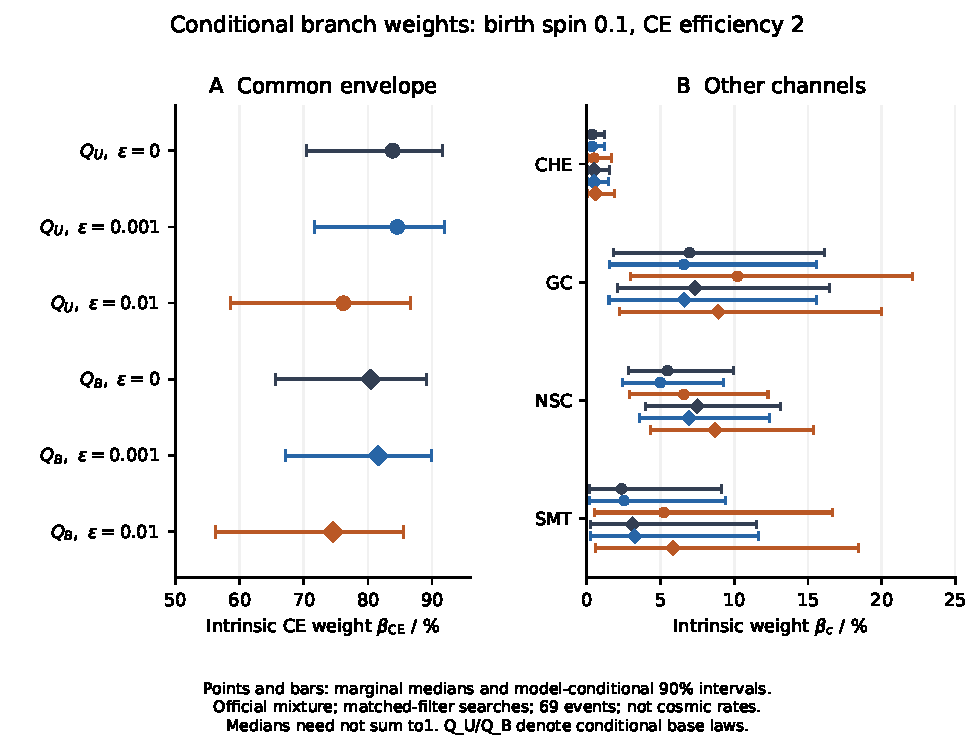
\includegraphics[width=\linewidth]{channel-posteriors.pdf}
\caption{六种明确模型条件下的五渠道后验。区间是模型内条件可信区间，不是已校准的总误差预算。全部69事件保留。}\label{fig:posterior}
\end{figure}

分支中位数沿正则器、补全、银行和搜索口径的最大移动分别为\MaxReg\ 个百分点（CE）、\MaxHidden\ 个百分点（CE）、\MaxBank\ 个百分点（CE）、\MaxPolicy\ 个百分点（NSC）。每个最大值在各自网格点取得，不能把它们当四个独立误差相加。特别是，早先描述性自旋模型中较小的银行变化，不能认证另一形成渠道模型。

均匀基准、官方混合银行下，CE从$\epsilon=0$的83.85\%变成$\epsilon=0.01$的76.17\%；它的检出\emph{标签}中位数在两者中都约为25\%。式\eqref{eq:decomposition}对这种比较必不可少。该补全下未正则化CE计算效率约0.00139，而$\xi_U\simeq0.08065$；因此1\%共同项能显著改变CE内禀与检出权重的转换。其检出混合责任份额中位数是12.14\%，不是1\%（图\ref{fig:sensitivity}）。这并不证明12\%的观测双星来自某个未知物理渠道。

在均匀基准、$\epsilon=0.001$、官方混合银行设定的后验均值处，GW190521的共同项责任份额约0.84；正则化前该事件的贡献集中诊断较低。这是模型尾部诊断，不是删除事件的理由，也不是独立测定的事件分类。

\begin{figure}[tb]
\centering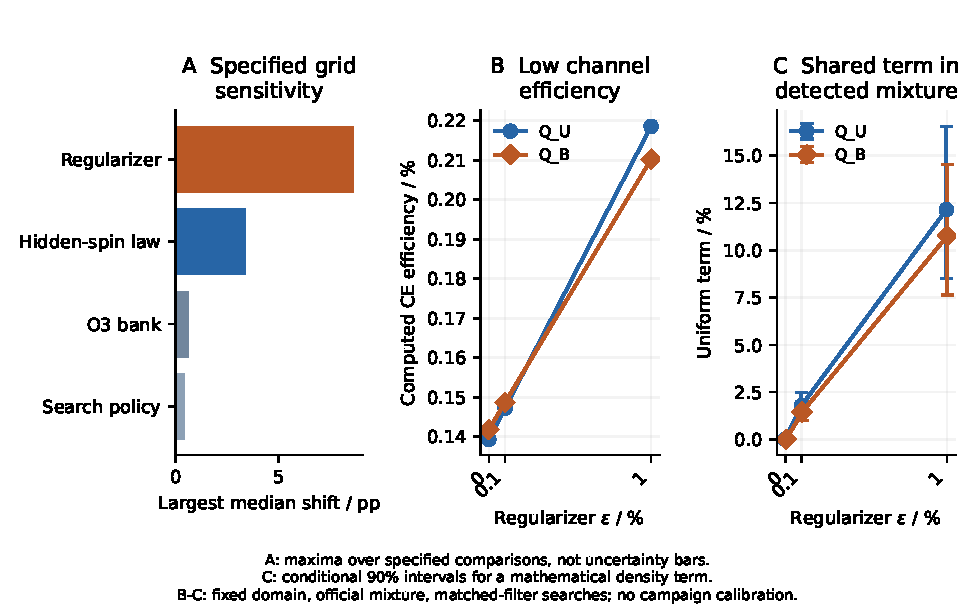
\includegraphics[width=\linewidth]{channel-sensitivity.pdf}
\caption{指定敏感性最大值及正则器的选择响应。共同项计算效率较高时，较小内禀概率能对应较大检出密度份额。C给出一个数学项的模型内条件区间，不是天体物理总体。}\label{fig:sensitivity}
\end{figure}

\section{尚未证明的部分}
给定保存积分时参数后验可以数值稳定，但这些积分仍未必是经校准的物理似然与选择近似。最小事件贡献集中量只有\MinEvent，最小选择集中量为\MinSelection。我们没有用ESS门槛删除这些设定；这些诊断和独立后验采样也都不修复有限银行尾部、PE链相关或未见支持。

限制是具体的：尚未推断出生自旋与CE效率，尚未重建各渠道真实隐藏自旋、完整历史注入协议、PE排除区域的似然、波形系统误差传播或真实活动覆盖率。log-alpha上下文是数据支持的解释，不是历史执行重建。限制域避开已知O3红移支持不匹配，却不约束被排除的宇宙总体。均匀正则器的坐标约定也是指定选择，不是唯一物理处方。这些缺口阻止全局形成比例或一般稳健性结论。

下一项实质检验是对本批\emph{渠道}积分做成对有限银行传播，尤其检查低集中事件及选择项，随后检验有物理动机的渠道特定自旋补全或更完整群体合成产品。不能把此前描述性模型的抽稀范围挪用到这里。

\section{复现与研究状态}
仓库保存固定设计、来源清单、模型产品校验和、全部69事件积分、选择矩、归一化、所有数值失败、后验重复和独立检查。从已有已核验缓存出发，依次运行渠道积分生产器、Decimal乘积校验、分支拟合、独立Metropolis验证、检出项拆分和汇总脚本。原始数据与权重需单独取得；这不是洁净环境一键复现。本文数值、表格、图均从已检查JSON生成，并在两语言版本间共享。原v0.3论文及冻结输入保留。

澄衡（Chengheng）是本项目协作AI助手使用的研究笔名。本计算稿未同行评审，不表示机构背书，也不表示已完成物理形成渠道测量。
\FloatBarrier
\clearpage
\begin{thebibliography}{9}
\bibitem{zevin} M. Zevin et al., One channel to rule them all? Constraining the origins of binary black holes using multiple formation pathways, Astrophys. J. \textbf{910}, 152 (2021), \href{https://arxiv.org/abs/2011.10057v2}{arXiv:2011.10057v2}.
\bibitem{colloms} S. Colloms, C. P. L. Berry, J. Veitch, and M. Zevin, Exploring the evolution of gravitational-wave emitters with efficient emulation: Constraining the origins of binary black holes using normalising flows (2025), \href{https://arxiv.org/abs/2503.03819v1}{arXiv:2503.03819v1}; model products: \href{https://zenodo.org/records/14967688}{Zenodo 14967688}.
\bibitem{callister} T. A. Callister, A Thesaurus for Common Priors in Gravitational-Wave Astronomy (2021), \href{https://arxiv.org/abs/2104.09508}{arXiv:2104.09508}.
\bibitem{miller} S. J. Miller, Z. Ko, T. A. Callister, and K. Chatziioannou, Gravitational waves carry information beyond effective spin parameters but it is hard to extract, Phys. Rev. D \textbf{109}, 104036 (2024), \href{https://arxiv.org/abs/2401.05613v2}{arXiv:2401.05613v2}.
\bibitem{plunkett} C. Plunkett et al., Spinformation: do gravitational-wave events carry information beyond effective spins? (2026), \href{https://arxiv.org/abs/2610.18973v1}{arXiv:2610.18973v1}.
\bibitem{lvk} R. Abbott et al. (LIGO Scientific, Virgo, and KAGRA Collaborations), The population of merging compact binaries inferred using gravitational waves through GWTC-3, Phys. Rev. X \textbf{13}, 011048 (2023), \href{https://arxiv.org/abs/2111.03634}{arXiv:2111.03634}.
\bibitem{iwaya} M. Iwaya, K. Kobayashi, S. Morisaki, K. Hotokezaka, and T. Kinugawa, Analytic joint priors of effective spin parameters and inference of the spin distribution of binary black holes, Phys. Rev. D \textbf{111}, 103046 (2025), \href{https://doi.org/10.1103/PhysRevD.111.103046}{doi:10.1103/PhysRevD.111.103046}.
\bibitem{vehtari} A. Vehtari, A. Gelman, D. Simpson, B. Carpenter, and P.-C. B\"urkner, Rank-normalization, folding, and localization: An improved $\widehat R$ for assessing convergence of MCMC, Bayesian Anal. \textbf{16}, 667 (2021), \href{https://arxiv.org/abs/1903.08008v5}{arXiv:1903.08008v5}.
\end{thebibliography}

